\section{Algorithms for content-based filtering}\label{sec:cbf_algorithms}
Content-based filtering could be used in a variety of contexts. Depending on the needs of a recommendation system we could have different implementations of CBF. Depending on data type, commonly used models include Naive Bayes classifier \cite{Naive_classifier}, K-Nearest Neighbors or neural networks.  The most popular and widely used methods are based on vector space, but there are also other techniques, like Decision-tree.

\subsection{Decision-tree method}
Decision-tree could be used not only with Content-based filtering, but also with other recommendation methods. It is not really popular due to several reasons, but could have advantages in specific situations. Decision-tree method relies on inductive learning, therefore we firstly should have some data from the user (his preferences or previous actions). After that, we could use algorithms like C4.5\cite{C4_5} or newer version C5.0. Given algorithm will produce a decision tree based on user preferences and it will be used as a user profile. The example of a decision tree is shown in Figure~\ref{fig:decision_tree}\cite{Decision_Tree}.

After construction of the decision tree, we can classify new items, with which the user has not yet interacted. If the item has similar categories (this approach could be used only if items have some sort of categorization) to those which are preferable to user profile, the output of the decision tree for these items would be abstract “Like”. This will mean that we could recommend a new item to a user with a high probability that this item will interest the user. The decision tree can be reconstructed during the process of interacting with new content which will improve the recommendation results.

However, this algorithm has some disadvantages. Firstly, the computational complexity of C4.5 during the training data is $\mathbf{O(m^2)}$. For a small amount of data it wouldn't be a problem, but if the user have been interacted with thousands of items, rebuilding the decision tree won't be a trivial task. Computational cost during the recommendation process is $\mathbf{O(n)}$, which also could be a problem with high amounts of presented items\cite{Decision_Tree}.
\begin{center}
    \begin{figure}[H]
    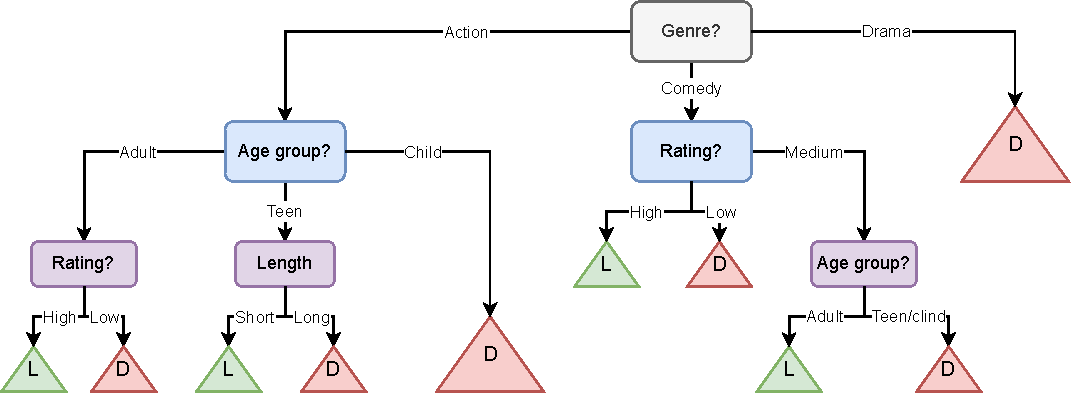
\includegraphics[width=\textwidth]{figures/diagrams/article_decision_tree_colored.pdf}
    \caption{Example of decision-tree}
    \label{fig:decision_tree}
    \end{figure}
\end{center}

\subsection{K-Nearest Neighbor method}
K-Nearest Neighbor (KNN) belongs to vector space methods that are used in N dimensional environments. It is highly used and has better results than decision-tree in the majority of data sets\cite{KNN}.

But before using KNN, we should collect data from user interactions (e.g. user likes) into a user-item matrix. The example of the user-item matrix is shown in Table \ref{tab:user_item_matrix}. In example, each user rated movies from 1 to 5. If the movie is not rated by a user, it has the value 0. Additionaly, we should organize our data (in this example, movies) and convert it to an array of numbers. The exact  algorithm depends on the solution and environment, therefore we couldn`t define it in general. However, in this example we will use genres to define similarities between items. If the movie has a specific genre, the value in the matrix would be 1, otherwise 0. An example of a genre matrix is illustrated in Table \ref{tab:genre_movie_matrix}.

\begin{table}[h]
    \centering
    \begin{tabular}{|c|c|c|c|c|}
        \hline
        \textbf{Users} & \textbf{Movie 1} & \textbf{Movie 2} & \textbf{Movie 3} & \textbf{Movie 4} \\        
        \hline
        User 1 & 3 & 0 & 1 & 2\\
        \hline
        User 2 & 0 & 5 & 5 & 3\\
        \hline
        User 3 & 5 & 1 & 1 & 2\\
        \hline
        User 4 & 0 & 0 & 5 & 0\\
        \hline
    \end{tabular}
    \caption{User-item matrix}\label{tab:user_item_matrix}
\end{table}

\begin{table}[h]
    \centering
    \begin{tabular}{|c|c|c|c|c|}
        \hline
        \textbf{Genres} & \textbf{Movie 1} & \textbf{Movie 2} & \textbf{Movie 3} & \textbf{Movie 4} \\        
        \hline
        Action  & 1 & 0 & 0 & 1\\
        \hline
        Romance & 0 & 1 & 1 & 0\\
        \hline
        Comedy  & 1 & 1 & 1 & 0\\
        \hline
        Horror  & 0 & 0 & 0 & 1\\
        \hline
    \end{tabular}
    \caption{Genre-movie matrix}\label{tab:genre_movie_matrix}
\end{table}

After creation of genre-movie matrix, It becomes possible to create a matrix of similarities between items. We could do it in several ways, using different equations of distances (Euclidean, Minkowsky, Manhattan distances \cite{Different_KNN_distances}), but in example cosine similarity will be used. This approach is not often used and has some disadvantages, but for some datasets it has better results \cite{Cosine_Similarity}. The cosine similarity equation is illustrated below.

\begin{equation}
    \text{similarity} = \cos(\theta) = \frac{\vec{A} \cdot \vec{B}}{||\vec{A}|| \times ||\vec{B}||} = \frac{\sum_{i=1}^{n} A_i B_i}{\sqrt{\sum_{i=1}^{n} A_i^2} \times \sqrt{\sum_{i=1}^{n} B_i^2}}\label{equ:cosine_similarity}
\end{equation}

The resulted matrix after using cosine similarity is showed in Table \ref{tab:cosine_similarity_matrix}. The higher the value, the more similar the elements are to each other.
\begin{table}[h]
    \centering
    \begin{tabular}{|c|c|c|c|c|}
        \hline
         & Movie 1 & Movie 2 & Movie 3 & Movie 4 \\        
        \hline
        Movie 1 &1		&0.5	&0.5	&0.5\\
        \hline	
        Movie 2 &0.5	&1      &1		&0	\\
        \hline
        Movie 3 &0.5	&1		&1		&0	\\
        \hline
        Movie 4 &0.5	&0		&0		&1	\\
        \hline
    \end{tabular}
    \caption{Cosine similarity matrix}\label{tab:cosine_similarity_matrix}
\end{table}

After preparatory processes, we can use the K-Nearest Neighbor algorithm to find similar unknown movies to the user based on rated items. For the second user, we can see that he rated the third movie 5, therefore we should find similar movies to the movie number 3. For the KNN algorithm we should define the number of elements which will be found. The exact number should be calculated through equations, but for this small dataset of 4 elements K equals to 2 would be fine. Due to the matrix of cosine similarity, two the nearest items to the third movie are first and second movies. Movie number 2 is more similar (It is the same), but the user has already rated this movie. Therefore, the output and recommended item would be movie number 1 with similarity of 0.5 .

K-Nearest Neighbor has overall complexity of  $\boldsymbol{O(3mn + n \log n)}$ \cite{KNN_complexity} which is higher than decision-tree method, with recommendation computational cost $\mathbf{O(n)}$. K-Nearest Neighbor does not require the creation of a tree, but it requires a distance matrix, therefore the creation process wouldn`t be really fast. However, K-Nearest Neighbor has modified versions like Approximate Nearest Neighbors (ANN) or K-Dimensional Tree (KD-Tree) that are much faster with similar efficiency \cite{KNN_modifications}.
